
The high precision vertex detector positioned very closely to the interaction point is followed by a hybrid tracking layout, realised as a combination of silicon tracking with a time projection chamber, and a calorimeter system. The complete system is located inside a large solenoid providing a magnetic field of 3.5-4 T. On the outside of the coil, the iron return yoke is instrumented as a muon system and as a tail catcher calorimeter. 
	
\thisfloatsetup{floatwidth=\SfigwFull,capposition=beside}
\begin{figure}[b!]
\begin{tabular}{cc}

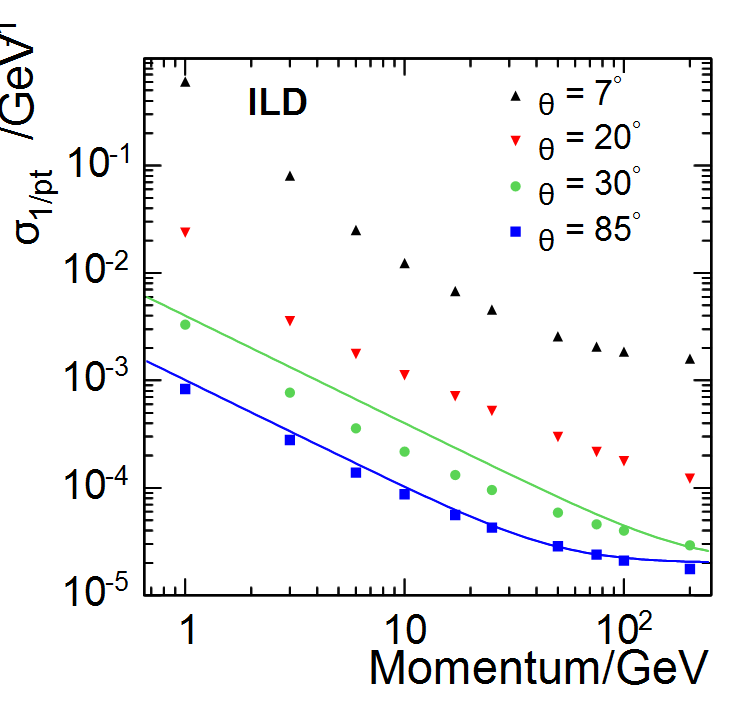
\includegraphics[width=0.5\hsize]{Introduction/fig/deltaInvP_all_fits.png} &
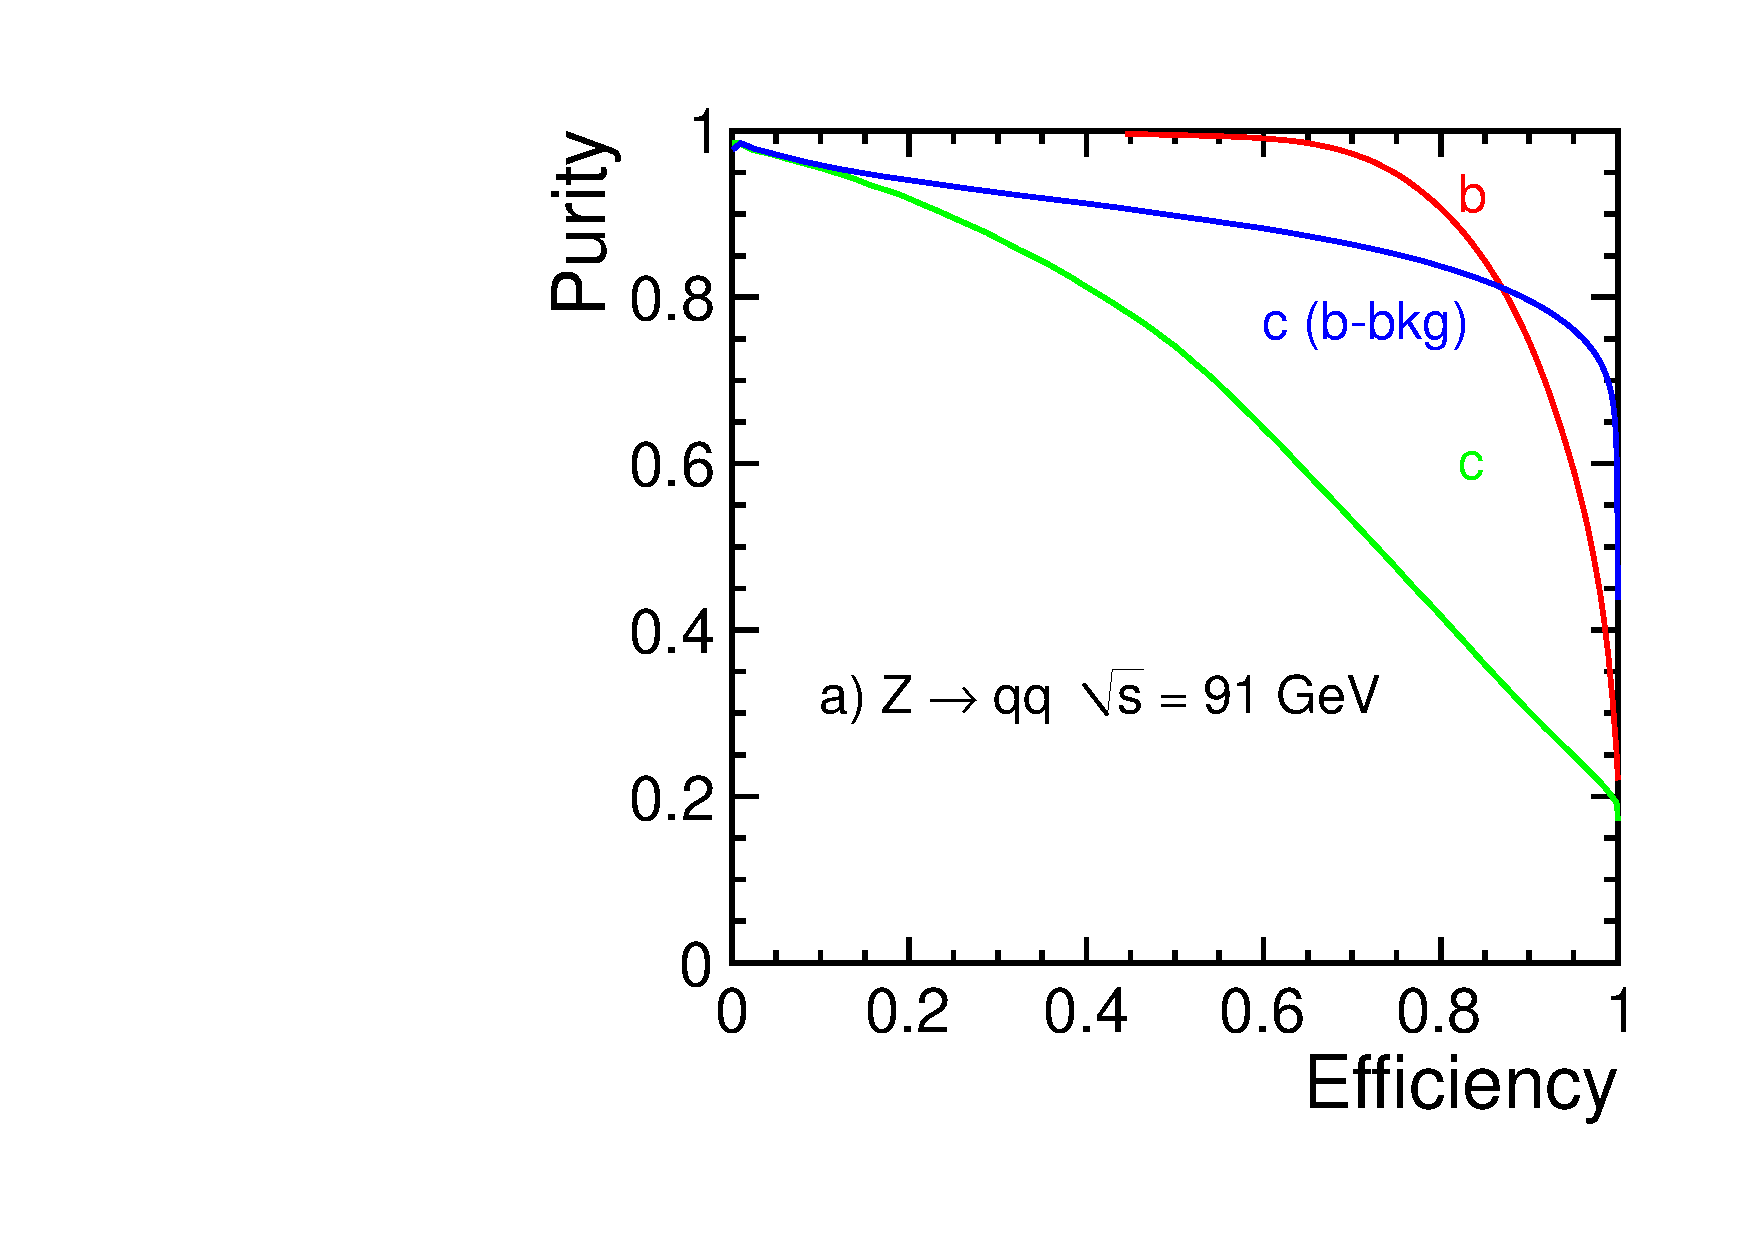
\includegraphics[width=0.5\hsize]{Introduction/fig/evalZ-lcfiweights_qq91new_v02-test.pdf}
\end{tabular}
\caption{\label{ild:fig:intro:tracking}(left) Momentum resolution for the ILD detector concept, as a function of the transverse momentum of the particle. (right) Flavour tagging efficiency versus purity for bottom events in sample of Z decays at 91\,GeV, and for charm events with only bottom background. )}
\end{figure}



\begin{figure}[t!]

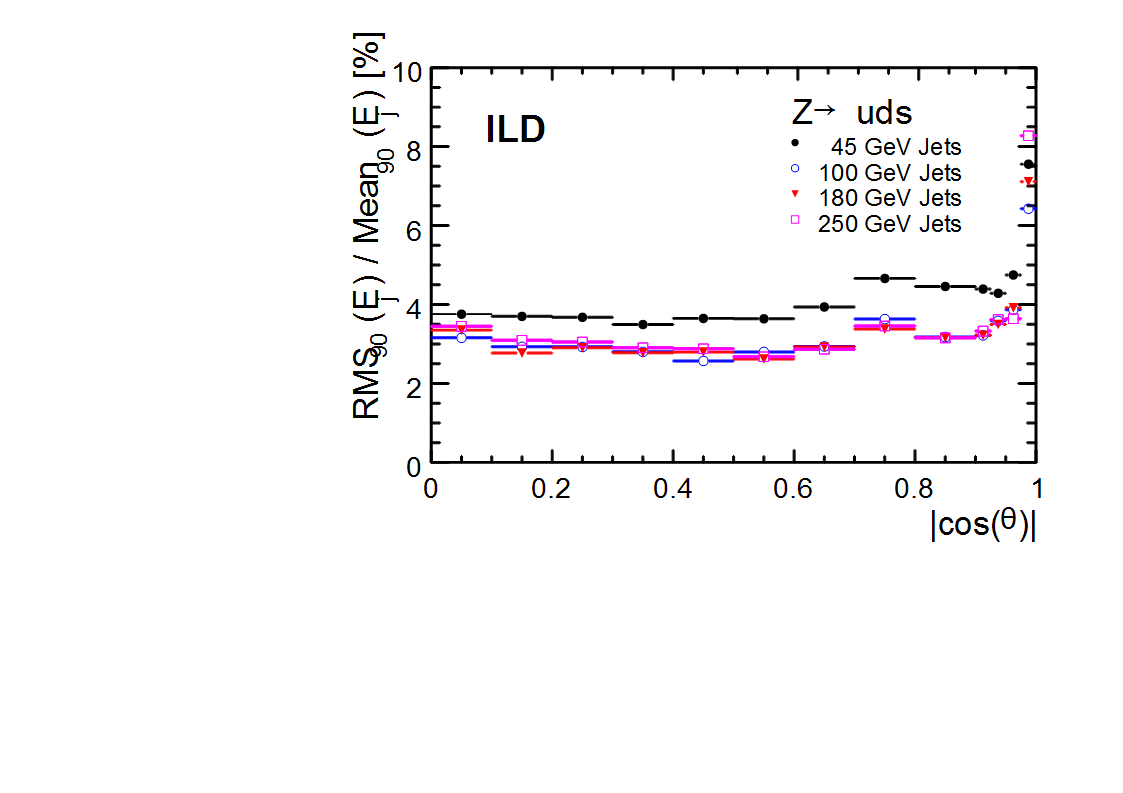
\includegraphics[width=0.8\hsize]{Introduction/fig/ild01_o1_pflow.png}

\caption{\label{ild:fig:intro:pflow}Fractional jet energy resolution
    plotted against $|\cos\theta|$ where theta is the polar angle of the thrust axis of the event. }
\end{figure}

The performance of the ILD concept has been extensively studied using a detailed GEANT4 based simulation model and sophisticated reconstruction tools. Backgrounds have been taken into account to the best of current knowledge.

The performance of the tracking system can be summarised by its combined momentum resolution, shown in Figure~\ref{ild:fig:intro:tracking}~(left). A resolution of $\sigma_{1/p_T} = 2 \times 10^{-5}$\,GeV$^{-1}$ has been achieved for high momenta. For many physics studies the tagging of long lived particles is of key importance. Several layers of pixel detectors close to the IP allow the reconstruction of displaced vertices, as shown in Figure~\ref{ild:fig:intro:tracking}~(right).

Calorimeter system and tracking system together enter into the particle flow performance. The performance of the ILD detector for different energies and as a function of the polar angle is shown in Figure~\ref{ild:fig:intro:pflow}. 

The few plots shown in this introduction illustrate the anticipated performance of the detector and illustrate the potential for precision measurements with the ILD detector. More details on the performance may be found in section~\ref{ild:sec:performance} of this document. 
